% Options for packages loaded elsewhere
\PassOptionsToPackage{unicode}{hyperref}
\PassOptionsToPackage{hyphens}{url}
%
\documentclass[
  a4paper,
]{article}
\usepackage{amsmath,amssymb}
\usepackage{iftex}
\ifPDFTeX
  \usepackage[T1]{fontenc}
  \usepackage[utf8]{inputenc}
  \usepackage{textcomp} % provide euro and other symbols
\else % if luatex or xetex
  \usepackage{unicode-math} % this also loads fontspec
  \defaultfontfeatures{Scale=MatchLowercase}
  \defaultfontfeatures[\rmfamily]{Ligatures=TeX,Scale=1}
\fi
\usepackage{lmodern}
\ifPDFTeX\else
  % xetex/luatex font selection
    \setmainfont[]{Helvetica}
\fi
% Use upquote if available, for straight quotes in verbatim environments
\IfFileExists{upquote.sty}{\usepackage{upquote}}{}
\IfFileExists{microtype.sty}{% use microtype if available
  \usepackage[]{microtype}
  \UseMicrotypeSet[protrusion]{basicmath} % disable protrusion for tt fonts
}{}
\makeatletter
\@ifundefined{KOMAClassName}{% if non-KOMA class
  \IfFileExists{parskip.sty}{%
    \usepackage{parskip}
  }{% else
    \setlength{\parindent}{0pt}
    \setlength{\parskip}{6pt plus 2pt minus 1pt}}
}{% if KOMA class
  \KOMAoptions{parskip=half}}
\makeatother
\usepackage{xcolor}
\usepackage[margin=0.75in]{geometry}
\usepackage{graphicx}
\makeatletter
\newsavebox\pandoc@box
\newcommand*\pandocbounded[1]{% scales image to fit in text height/width
  \sbox\pandoc@box{#1}%
  \Gscale@div\@tempa{\textheight}{\dimexpr\ht\pandoc@box+\dp\pandoc@box\relax}%
  \Gscale@div\@tempb{\linewidth}{\wd\pandoc@box}%
  \ifdim\@tempb\p@<\@tempa\p@\let\@tempa\@tempb\fi% select the smaller of both
  \ifdim\@tempa\p@<\p@\scalebox{\@tempa}{\usebox\pandoc@box}%
  \else\usebox{\pandoc@box}%
  \fi%
}
% Set default figure placement to htbp
\def\fps@figure{htbp}
\makeatother
\setlength{\emergencystretch}{3em} % prevent overfull lines
\providecommand{\tightlist}{%
  \setlength{\itemsep}{0pt}\setlength{\parskip}{0pt}}
\setcounter{secnumdepth}{-\maxdimen} % remove section numbering
\usepackage{titling}
\pretitle{\begin{flushleft}}
\posttitle{\end{flushleft}}
\usepackage{booktabs}
\usepackage{longtable}
\usepackage{float}
\floatplacement{figure}{H}
\usepackage{colortbl}
\usepackage{pdflscape}
\usepackage{tabu}
\usepackage{makecell}
\usepackage{xcolor}
\usepackage{soul}
\usepackage{caption}
\usepackage[singlelinecheck=false]{caption}
\usepackage[font={small,bf}]{caption}
\usepackage{multirow}
\usepackage{array}
\usepackage{lscape}
\newcommand{\blandscape}{\begin{landscape}}
\newcommand{\elandscape}{\end{landscape}}
\usepackage[dvipsnames]{xcolor}
\renewcommand{\footnotesize}{\tiny}
\usepackage{threeparttable}
\usepackage{booktabs}
\usepackage{longtable}
\usepackage{array}
\usepackage{multirow}
\usepackage{wrapfig}
\usepackage{float}
\usepackage{colortbl}
\usepackage{pdflscape}
\usepackage{tabu}
\usepackage{threeparttable}
\usepackage{threeparttablex}
\usepackage[normalem]{ulem}
\usepackage{makecell}
\usepackage{xcolor}
\usepackage{bookmark}
\IfFileExists{xurl.sty}{\usepackage{xurl}}{} % add URL line breaks if available
\urlstyle{same}
\hypersetup{
  hidelinks,
  pdfcreator={LaTeX via pandoc}}

\title{\vspace{-1.5cm} \begin{LARGE} WGS Quality Control Report \end{LARGE}}
\author{}
\date{\vspace{-2.5em}}

\begin{document}
\maketitle

\normalsize Batch Name: 2025-06-27\_P

\normalsize Experiment Name: 25ARS\_KPNGHRU\_LY9BB

\fontsize{7}{8}
\selectfont
\captionsetup[table]{labelformat=empty}
\renewcommand{\arraystretch}{1.2}

\begin{longtable}[t]{>{\centering\arraybackslash}p{1cm}>{\centering\arraybackslash}p{2.8cm}>{\centering\arraybackslash}p{1.5cm}>{\centering\arraybackslash}p{5cm}>{\centering\arraybackslash}p{5cm}}
\toprule
\multicolumn{1}{>{\centering\arraybackslash}p{1cm}}{\cellcolor[HTML]{D4D4D4}{\textbf{Isolate No.}}} & \multicolumn{1}{>{\centering\arraybackslash}p{2.8cm}}{\cellcolor[HTML]{D4D4D4}{\textbf{Sample ID}}} & \multicolumn{1}{>{\centering\arraybackslash}p{1.5cm}}{\cellcolor[HTML]{D4D4D4}{\textbf{Description}}} & \multicolumn{1}{>{\centering\arraybackslash}p{5cm}}{\cellcolor[HTML]{D4D4D4}{\textbf{ARSRL}}} & \multicolumn{1}{>{\centering\arraybackslash}p{5cm}}{\cellcolor[HTML]{D4D4D4}{\textbf{WGS}}}\\
\midrule
1 & UTPN\_BL0001 & UDI166 & \em{Escherichia coli} & \em{Escherichia coli}\\
2 & 24ARS\_MMH0020 & UDI105 & \em{Klebsiella pneumoniae} & \em{Klebsiella pneumoniae}\\
3 & 24ARS\_VSM0631 & UDI104 & \em{Klebsiella pneumoniae} & \em{Klebsiella pneumoniae}\\
4 & 25ARS\_BGH0054 & UDI098 & \em{Klebsiella pneumoniae} & \em{Klebsiella pneumoniae}\\
5 & 25ARS\_BGH0055 & UDI099 & \em{Klebsiella pneumoniae} & \em{Klebsiella pneumoniae}\\
\addlinespace
6 & 25ARS\_BGH0057 & UDI103 & \em{Klebsiella pneumoniae} & \em{Klebsiella pneumoniae}\\
7 & 25ARS\_BGH0058 & UDI100 & \em{Klebsiella pneumoniae} & \em{Klebsiella pneumoniae}\\
8 & 25ARS\_BGH0059 & UDI101 & \em{Klebsiella pneumoniae} & \em{Klebsiella pneumoniae}\\
9 & 25ARS\_BRT0014 & UDI192 & \em{Klebsiella pneumoniae} & \em{Klebsiella pneumoniae}\\
10 & 25ARS\_BRT0015 & UDI097 & \em{Klebsiella pneumoniae} & \em{Klebsiella pneumoniae}\\
\addlinespace
11 & 25ARS\_CVM0013 & UDI108 & \em{Klebsiella pneumoniae} & \em{Klebsiella pneumoniae}\\
12 & 25ARS\_CVM0014 & UDI109 & \em{Klebsiella pneumoniae} & \em{Klebsiella pneumoniae}\\
13 & 25ARS\_EVR0016 & UDI191 & \em{Klebsiella pneumoniae} & \em{Klebsiella pneumoniae}\\
14 & 25ARS\_JLM0010 & UDI106 & \em{Klebsiella pneumoniae} & \em{Klebsiella pneumoniae}\\
15 & 25ARS\_JLM0011 & UDI107 & \em{Klebsiella pneumoniae} & \em{Klebsiella pneumoniae}\\
\addlinespace
\cellcolor[HTML]{FD7979}{16} & \cellcolor[HTML]{FD7979}{25ARS\_JLM0021} & \cellcolor[HTML]{FD7979}{UDI110} & \cellcolor[HTML]{FD7979}{\em{Klebsiella pneumoniae}} & \cellcolor[HTML]{FD7979}{\em{Klebsiella pneumoniae}}\\
17 & 25ARS\_NKI0002 & UDI112 & \em{Klebsiella pneumoniae} & \em{Klebsiella pneumoniae}\\
18 & 25ARS\_NKI0003 & UDI165 & \em{Klebsiella pneumoniae} & \em{Klebsiella pneumoniae}\\
19 & 25ARS\_MAR0024 & UDI102 & \em{Klebsiella pneumoniae} & \em{Klebsiella variicola}\\
20 & 25ARS\_VC0029 & UDI167 & \em{Neisseria gonorrhoeae} & \em{Neisseria gonorrhoeae}\\
\addlinespace
21 & 25ARS\_VC0029 & UDI168 & \em{Neisseria gonorrhoeae} & \em{Neisseria gonorrhoeae}\\
22 & 25ARS\_MAR0025 & UDI111 & \em{Klebsiella pneumoniae (x)} & \em{Raoultella planticola}\\
\bottomrule
\multicolumn{5}{l}{\rule{0pt}{1em}\textit{Legend:} PASS   |   \colorbox{Salmon}{FAILURE}   |   \textcolor{Blue}{EXCEEDS THRESHOLD METRIC/S}   |   (x) - NON-CONCORDANT   |}\\
\end{longtable}

\fontsize{7}{8}
\selectfont
\captionsetup[table]{labelformat=empty}
\renewcommand{\arraystretch}{1.2}

\(\\\) \newpage

\begin{landscape}
\fontsize{7}{8}
\selectfont
\captionsetup[table]{labelformat=empty}
\renewcommand{\arraystretch}{1.2}

\begin{table}[!h]
\centering
\resizebox{\ifdim\width>\linewidth\linewidth\else\width\fi}{!}{
\begin{tabular}{cc>{}ccccccccc}
\toprule
\cellcolor[HTML]{D4D4D4}{\textbf{Isolate No.}} & \cellcolor[HTML]{D4D4D4}{\textbf{Sample ID}} & \cellcolor[HTML]{D4D4D4}{\textbf{WGS ID}} & \cellcolor[HTML]{D4D4D4}{\textbf{completeness}} & \cellcolor[HTML]{D4D4D4}{\textbf{contamination}} & \cellcolor[HTML]{D4D4D4}{\textbf{Depth of coverage}} & \cellcolor[HTML]{D4D4D4}{\textbf{Genome size}} & \cellcolor[HTML]{D4D4D4}{\textbf{GC content}} & \cellcolor[HTML]{D4D4D4}{\textbf{Contig count}} & \cellcolor[HTML]{D4D4D4}{\textbf{N50}} & \cellcolor[HTML]{D4D4D4}{\textbf{Mean read Q-score}}\\
\midrule
1 & UTPN\_BL0001 & \em{Escherichia coli} & 100 & 1.88 & 36.6 & 5.30 Mb & 50.62 & 113 & 165049 & 36.4\\
2 & 24ARS\_MMH0020 & \em{Klebsiella pneumoniae} & 100 & 0.14 & 66.5 & 5.16 Mb & 58.06 & 25 & 806509 & 36.2\\
3 & 24ARS\_VSM0631 & \em{Klebsiella pneumoniae} & 100 & 0.16 & 58.1 & 5.34 Mb & 57.41 & 107 & 136190 & 35.8\\
4 & 25ARS\_BGH0054 & \em{Klebsiella pneumoniae} & 100 & 0.24 & 60.2 & 5.31 Mb & 57.36 & 34 & 383019 & 36.0\\
5 & 25ARS\_BGH0055 & \em{Klebsiella pneumoniae} & 100 & 0.07 & 114.4 & 5.19 Mb & 57.65 & 28 & 372904 & 36.2\\
\addlinespace
6 & 25ARS\_BGH0057 & \em{Klebsiella pneumoniae} & 100 & 0.63 & 76.1 & 5.38 Mb & 57.22 & 87 & 170931 & 35.9\\
7 & 25ARS\_BGH0058 & \em{Klebsiella pneumoniae} & 100 & 0.28 & 142.2 & 5.52 Mb & 57.16 & 41 & 274455 & 36.0\\
8 & 25ARS\_BGH0059 & \em{Klebsiella pneumoniae} & 100 & 0.04 & 37.0 & 5.17 Mb & 57.67 & 32 & 412159 & 35.9\\
9 & 25ARS\_BRT0014 & \em{Klebsiella pneumoniae} & 100 & 2.2 & 64.6 & 5.57 Mb & 57.06 & 60 & 234586 & 35.7\\
10 & 25ARS\_BRT0015 & \em{Klebsiella pneumoniae} & 100 & 0.25 & 36.3 & 5.48 Mb & 57.3 & 57 & 372661 & 36.1\\
\addlinespace
11 & 25ARS\_CVM0013 & \em{Klebsiella pneumoniae} & 100 & 0.28 & 60.0 & 5.45 Mb & 57.18 & 42 & 301992 & 35.9\\
12 & 25ARS\_CVM0014 & \em{Klebsiella pneumoniae} & 100 & 0.18 & 44.6 & 5.59 Mb & 57.3 & 46 & 327262 & 36.1\\
13 & 25ARS\_EVR0016 & \em{Klebsiella pneumoniae} & 100 & 1.03 & 20.9 & 5.54 Mb & 57.22 & 86 & 258346 & 35.9\\
14 & 25ARS\_JLM0010 & \em{Klebsiella pneumoniae} & 100 & 1.09 & 76.5 & 5.52 Mb & 57.27 & 42 & 403130 & 36.1\\
15 & 25ARS\_JLM0011 & \em{Klebsiella pneumoniae} & 100 & 0.28 & 37.8 & 5.49 Mb & 57.12 & 57 & 444699 & 35.9\\
\addlinespace
\cellcolor[HTML]{FD7979}{16} & \cellcolor[HTML]{FD7979}{25ARS\_JLM0021} & \em{\cellcolor[HTML]{FD7979}{Klebsiella pneumoniae}} & \cellcolor[HTML]{FD7979}{100} & \cellcolor[HTML]{FD7979}{0.39} & \cellcolor[HTML]{FD7979}{\textcolor{blue}{\textbf{ 17.7}}} & \cellcolor[HTML]{FD7979}{5.40 Mb} & \cellcolor[HTML]{FD7979}{57.32} & \cellcolor[HTML]{FD7979}{125} & \cellcolor[HTML]{FD7979}{91290} & \cellcolor[HTML]{FD7979}{36.1}\\
17 & 25ARS\_NKI0002 & \em{Klebsiella pneumoniae} & 100 & 0.13 & 24.6 & 5.29 Mb & 57.37 & 44 & 482736 & 35.5\\
18 & 25ARS\_NKI0003 & \em{Klebsiella pneumoniae} & 100 & 0.03 & 64.1 & 5.13 Mb & 58.02 & 25 & 780757 & 35.7\\
19 & 25ARS\_MAR0024 & \em{Klebsiella variicola} & 100 & 0.59 & 112.6 & 5.53 Mb & 57.27 & 29 & 498455 & 36.0\\
20 & 25ARS\_VC0029 & \em{Neisseria gonorrhoeae} & 100 & 0.15 & 152.3 & 2.14 Mb & 52.49 & 79 & 59587 & 35.9\\
\addlinespace
21 & 25ARS\_VC0029 & \em{Neisseria gonorrhoeae} & 100 & 0.15 & 156.4 & 2.14 Mb & 52.49 & 78 & 64416 & 35.8\\
22 & 25ARS\_MAR0025 & \em{Raoultella planticola} & 100 & 1.54 & 35.4 & 5.56 Mb & 55.78 & 49 & 268070 & 36.2\\
\bottomrule
\multicolumn{11}{l}{\rule{0pt}{1em}\textit{Legend:} PASS   |   \colorbox{Salmon}{FAILURE}   |   \textcolor{Blue}{EXCEEDS THRESHOLD METRIC/S}   |   (x) - NON-CONCORDANT   |}\\
\end{tabular}}
\end{table}









$\\$ $\\$ $\\$ $\color{red}{\normalsize\textbf{RECOMMENDATION:}}$



\begin{tabular}{>{\raggedright\arraybackslash}p{6cm}>{\centering\arraybackslash}p{6cm}>{\centering\arraybackslash}p{4cm}}
\toprule
\cellcolor[HTML]{D4D4D4}{\textbf{Sample ID}} & \cellcolor[HTML]{D4D4D4}{\textbf{Reason - Failed Metrics}} & \cellcolor[HTML]{D4D4D4}{\textbf{Remarks}}\\
\midrule
\cellcolor{gray!10}{25ARS\_JLM0021} & \cellcolor{gray!10}{Depth of coverage} & \cellcolor{gray!10}{For repeat testing}\\
25ARS\_MAR0025 & NA & Non-concordant result - Check Label\\
\bottomrule
\end{tabular}



\end{landscape}

\fontsize{7}{8}
\selectfont
\captionsetup[table]{labelformat=empty}
\renewcommand{\arraystretch}{1.2}

\begin{longtable}[l]{>{\raggedright\arraybackslash}p{8cm}c}
\toprule
\cellcolor[HTML]{D4D4D4}{\textbf{WGS\_ID}} & \cellcolor[HTML]{D4D4D4}{\textbf{Number}}\\
\midrule
\em{Klebsiella pneumoniae} & 17\\
\em{Neisseria gonorrhoeae} & 2\\
\em{Escherichia coli} & 1\\
\em{Klebsiella variicola} & 1\\
\em{Raoultella planticola} & 1\\
\bottomrule
\end{longtable}

\begin{itemize}
\item
  \(\color{red}5\) distinct species were identified among
  \(\color{red}22\) isolates.
\item
  \(\color{red}95.45\) \% (n=21) of the isolates passed the QC, while
  \(\color{red}4.55\) \% (n=1) were tagged with failure.
\item
  Concordance between ARSRL and WGS species report was
  \(\color{red}95.45\) \%. \(\\\)
\end{itemize}

\subsubsection{GRAPHS}\label{graphs}

\fontsize{7}{8}
\selectfont
\captionsetup[table]{labelformat=empty}
\renewcommand{\arraystretch}{1.2}

\pandocbounded{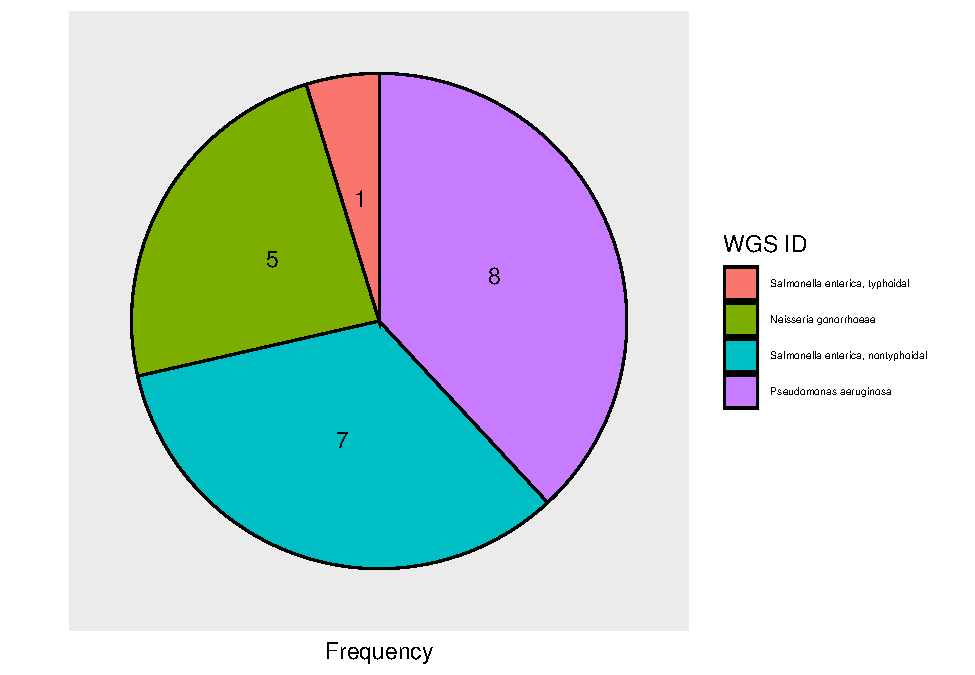
\includegraphics[keepaspectratio]{qualifyr_report_2025-06-27_P_files/figure-latex/pie_chart-1.pdf}}

\subsubsection{Result Classification}\label{result-classification}

\pandocbounded{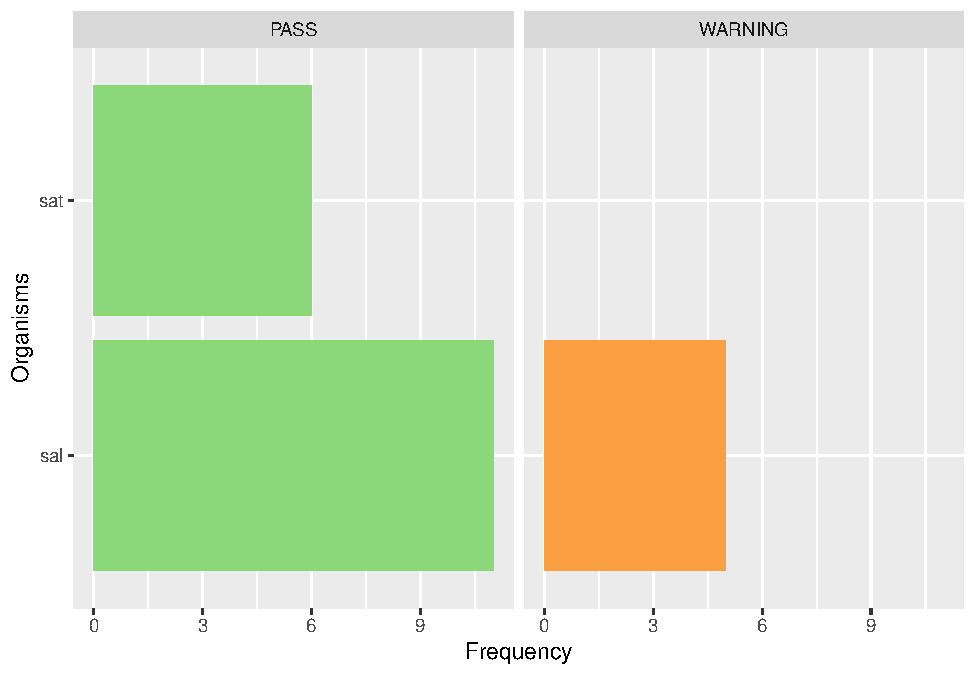
\includegraphics[keepaspectratio]{qualifyr_report_2025-06-27_P_files/figure-latex/organism results-1.pdf}}

\subsubsection{Number of contigs}\label{number-of-contigs}

\pandocbounded{\includegraphics[keepaspectratio]{qualifyr_report_2025-06-27_P_files/figure-latex/contigs_result-1.pdf}}

\subsubsection{N50 Value}\label{n50-value}

\pandocbounded{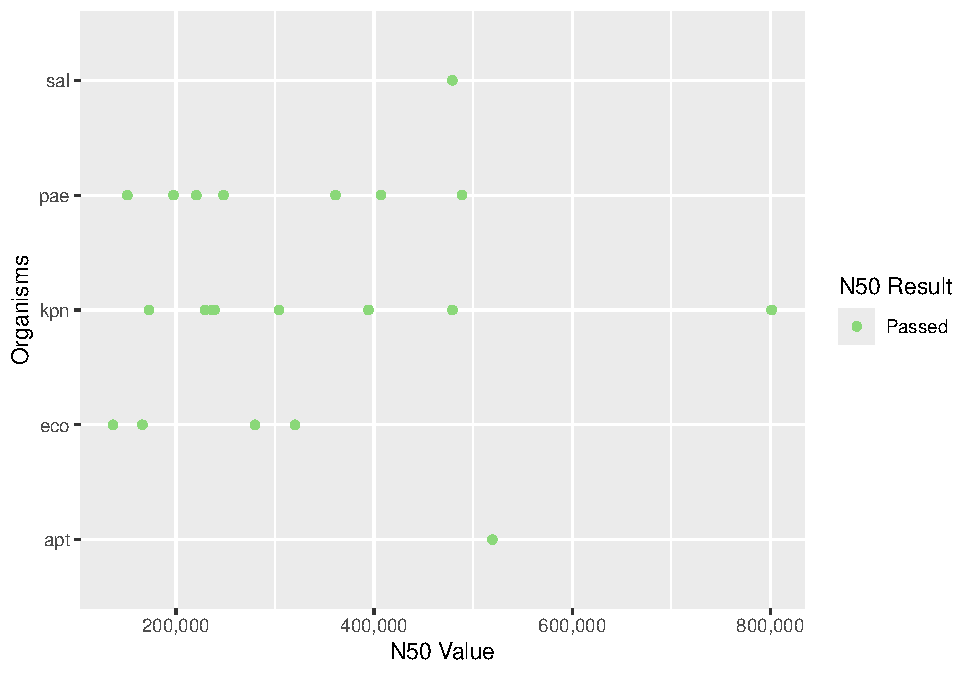
\includegraphics[keepaspectratio]{qualifyr_report_2025-06-27_P_files/figure-latex/n50_result -1.pdf}}

\subsubsection{Total Length}\label{total-length}

\pandocbounded{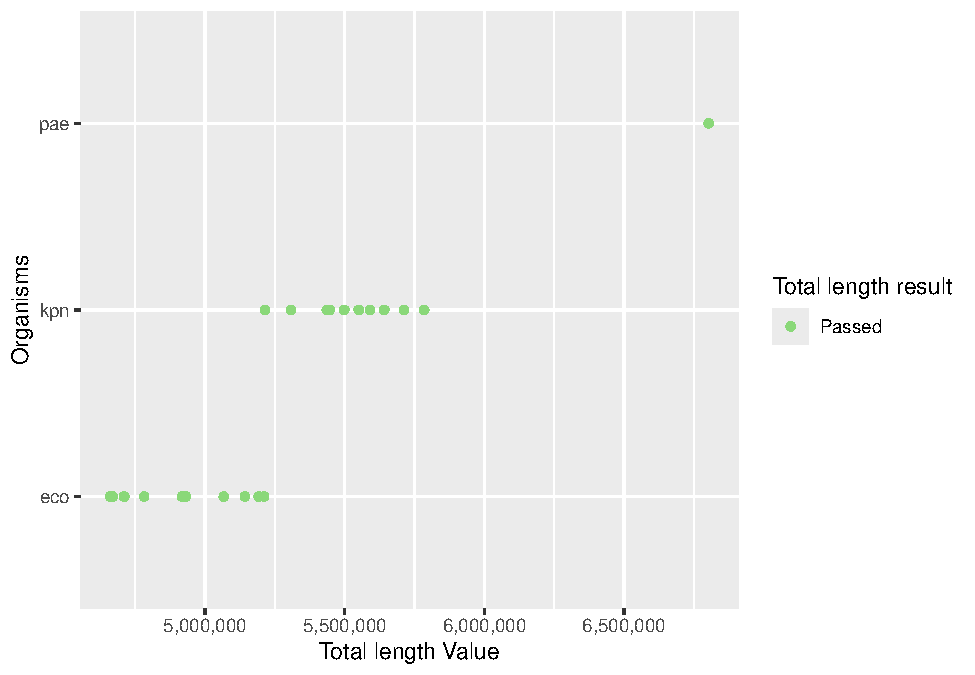
\includegraphics[keepaspectratio]{qualifyr_report_2025-06-27_P_files/figure-latex/length_result -1.pdf}}

\fontsize{7}{8}
\selectfont
\captionsetup[table]{labelformat=empty}
\renewcommand{\arraystretch}{1}

\subsubsection{MLST RESULTS}\label{mlst-results}

\begin{longtable}[l]{>{\centering\arraybackslash}p{3cm}>{\centering\arraybackslash}p{3cm}>{\centering\arraybackslash}p{1cm}>{\centering\arraybackslash}p{1cm}>{\centering\arraybackslash}p{1cm}>{\centering\arraybackslash}p{1cm}>{\centering\arraybackslash}p{1cm}>{\centering\arraybackslash}p{1cm}>{\centering\arraybackslash}p{1cm}>{\centering\arraybackslash}p{1cm}}
\toprule
\cellcolor[HTML]{D4D4D4}{\textbf{sample\_id}} & \cellcolor[HTML]{D4D4D4}{\textbf{species}} & \cellcolor[HTML]{D4D4D4}{\textbf{MLST}} & \cellcolor[HTML]{D4D4D4}{\textbf{gapA}} & \cellcolor[HTML]{D4D4D4}{\textbf{infB}} & \cellcolor[HTML]{D4D4D4}{\textbf{mdh}} & \cellcolor[HTML]{D4D4D4}{\textbf{pgi}} & \cellcolor[HTML]{D4D4D4}{\textbf{phoE}} & \cellcolor[HTML]{D4D4D4}{\textbf{rpoB}} & \cellcolor[HTML]{D4D4D4}{\textbf{tonB}}\\
\midrule
24ARS\_MMH0020 & \em{Klebsiella pneumoniae} & 2650 & 42 & 23 & 25 & 59 & 11 & 38 & 99\\
24ARS\_VSM0631 & \em{Klebsiella pneumoniae} & 5822 & 2 & 6 & 2 & 385 & 12 & 1 & 4\\
25ARS\_BGH0054 & \em{Klebsiella pneumoniae} & 186 & 2 & 1 & 1 & 37 & 45 & 4 & 9\\
25ARS\_BGH0055 & \em{Klebsiella pneumoniae} & 1516 & 2 & 6 & 10 & 1 & 20 & 10 & 25\\
25ARS\_BGH0057 & \em{Klebsiella pneumoniae} & 2882 & 2 & 3 & 1 & 1 & 7 & 1 & 13\\
\addlinespace
25ARS\_BGH0058 & \em{Klebsiella pneumoniae} & 35 & 2 & 1 & 2 & 1 & 10 & 1 & 19\\
25ARS\_BGH0059 & \em{Klebsiella pneumoniae} & 60 & 2 & 1 & 2 & 1 & 4 & 4 & 8\\
25ARS\_BRT0014 & \em{Klebsiella pneumoniae} & 147 & 3 & 4 & 6 & 1 & 7 & 4 & 38\\
25ARS\_BRT0015 & \em{Klebsiella pneumoniae} & 307 & 4 & 1 & 2 & 52 & 1 & 1 & 7\\
25ARS\_CVM0013 & \em{Klebsiella pneumoniae} & 35 & 2 & 1 & 2 & 1 & 10 & 1 & 19\\
\addlinespace
25ARS\_CVM0014 & \em{Klebsiella pneumoniae} & 23 & 2 & 1 & 1 & 1 & 9 & 4 & 12\\
25ARS\_EVR0016 & \em{Klebsiella pneumoniae} & 260 & 2 & 1 & 1 & 46 & 9 & 1 & 12\\
25ARS\_JLM0010 & \em{Klebsiella pneumoniae} & 23 & 2 & 1 & 1 & 1 & 9 & 4 & 12\\
25ARS\_JLM0011 & \em{Klebsiella pneumoniae} & 147 & 3 & 4 & 6 & 1 & 7 & 4 & 38\\
25ARS\_JLM0021 & \em{Klebsiella pneumoniae} & 2385 & 2 & 1 & 65 & 2 & 5 & 1 & 350\\
\addlinespace
25ARS\_MAR0024 & \em{Klebsiella variicola} & 3565 & 16 & 24 & 21 & 40 & 76 & 22 & 67\\
25ARS\_NKI0002 & \em{Klebsiella pneumoniae} & 432 & 4 & 1 & 1 & 2 & 7 & 4 & 4\\
25ARS\_NKI0003 & \em{Klebsiella pneumoniae} & - & 18 & 22 & 64 & 16 & \textasciitilde{}11 & 20 & 228\\
\bottomrule
\multicolumn{10}{l}{\rule{0pt}{1em}\textit{Legend: } (-) Not identified}\\
\end{longtable}

\begin{longtable}[l]{>{\centering\arraybackslash}p{3cm}>{\centering\arraybackslash}p{3cm}>{\centering\arraybackslash}p{1cm}>{\centering\arraybackslash}p{1cm}>{\centering\arraybackslash}p{1cm}>{\centering\arraybackslash}p{1cm}>{\centering\arraybackslash}p{1cm}>{\centering\arraybackslash}p{1cm}>{\centering\arraybackslash}p{1cm}>{\centering\arraybackslash}p{1cm}}
\toprule
\cellcolor[HTML]{D4D4D4}{\textbf{sample\_id}} & \cellcolor[HTML]{D4D4D4}{\textbf{species}} & \cellcolor[HTML]{D4D4D4}{\textbf{MLST}} & \cellcolor[HTML]{D4D4D4}{\textbf{gapA}} & \cellcolor[HTML]{D4D4D4}{\textbf{infB}} & \cellcolor[HTML]{D4D4D4}{\textbf{mdh}} & \cellcolor[HTML]{D4D4D4}{\textbf{pgi}} & \cellcolor[HTML]{D4D4D4}{\textbf{phoE}} & \cellcolor[HTML]{D4D4D4}{\textbf{rpoB}} & \cellcolor[HTML]{D4D4D4}{\textbf{tonB}}\\
\midrule
25ARS\_MAR0025 & \em{Raoultella planticola} & - & \textasciitilde{}31 & 47 & 65 & 37? & \textasciitilde{}93 & \textasciitilde{}44 & 40?\\
\bottomrule
\multicolumn{10}{l}{\rule{0pt}{1em}\textit{Legend: } (-) Not identified}\\
\end{longtable}

\begin{longtable}[l]{>{\centering\arraybackslash}p{3cm}>{\centering\arraybackslash}p{3cm}>{\centering\arraybackslash}p{1cm}>{\centering\arraybackslash}p{1cm}>{\centering\arraybackslash}p{1cm}>{\centering\arraybackslash}p{1cm}>{\centering\arraybackslash}p{1cm}>{\centering\arraybackslash}p{1cm}>{\centering\arraybackslash}p{1cm}>{\centering\arraybackslash}p{1cm}}
\toprule
\cellcolor[HTML]{D4D4D4}{\textbf{sample\_id}} & \cellcolor[HTML]{D4D4D4}{\textbf{species}} & \cellcolor[HTML]{D4D4D4}{\textbf{MLST}} & \cellcolor[HTML]{D4D4D4}{\textbf{gapA}} & \cellcolor[HTML]{D4D4D4}{\textbf{infB}} & \cellcolor[HTML]{D4D4D4}{\textbf{mdh}} & \cellcolor[HTML]{D4D4D4}{\textbf{pgi}} & \cellcolor[HTML]{D4D4D4}{\textbf{phoE}} & \cellcolor[HTML]{D4D4D4}{\textbf{rpoB}} & \cellcolor[HTML]{D4D4D4}{\textbf{tonB}}\\
\midrule
25ARS\_VC0029 & \em{Neisseria gonorrhoeae} & 7827 & 59 & 39 & 67 & 158 & 148 & 153 & \vphantom{1} 65\\
25ARS\_VC0029 & \em{Neisseria gonorrhoeae} & 7827 & 59 & 39 & 67 & 158 & 148 & 153 & 65\\
\bottomrule
\multicolumn{10}{l}{\rule{0pt}{1em}\textit{Legend: } (-) Not identified}\\
\end{longtable}

\begin{longtable}[l]{>{\centering\arraybackslash}p{3cm}>{\centering\arraybackslash}p{3cm}>{\centering\arraybackslash}p{1cm}>{\centering\arraybackslash}p{1cm}>{\centering\arraybackslash}p{1cm}>{\centering\arraybackslash}p{1cm}>{\centering\arraybackslash}p{1cm}>{\centering\arraybackslash}p{1cm}>{\centering\arraybackslash}p{1cm}>{\centering\arraybackslash}p{1cm}}
\toprule
\cellcolor[HTML]{D4D4D4}{\textbf{sample\_id}} & \cellcolor[HTML]{D4D4D4}{\textbf{species}} & \cellcolor[HTML]{D4D4D4}{\textbf{MLST}} & \cellcolor[HTML]{D4D4D4}{\textbf{gapA}} & \cellcolor[HTML]{D4D4D4}{\textbf{infB}} & \cellcolor[HTML]{D4D4D4}{\textbf{mdh}} & \cellcolor[HTML]{D4D4D4}{\textbf{pgi}} & \cellcolor[HTML]{D4D4D4}{\textbf{phoE}} & \cellcolor[HTML]{D4D4D4}{\textbf{rpoB}} & \cellcolor[HTML]{D4D4D4}{\textbf{tonB}}\\
\midrule
UTPN\_BL0001 & \em{Escherichia coli} & 131 & 53 & 40 & 47 & 13 & 36 & 28 & 29\\
\bottomrule
\multicolumn{10}{l}{\rule{0pt}{1em}\textit{Legend: } (-) Not identified}\\
\end{longtable}

\subsubsection{MLST RESULTS SUMMARY:}\label{mlst-results-summary}

\begin{longtable}[l]{>{\raggedright\arraybackslash}p{6cm}>{\raggedright\arraybackslash}p{10cm}}
\toprule
\cellcolor[HTML]{D4D4D4}{\textbf{wgs\_id}} & \cellcolor[HTML]{D4D4D4}{\textbf{mlst\_count}}\\
\midrule
\em{Klebsiella pneumoniae} & 2650 (n= 1 ), 5822 (n= 1 ), 186 (n= 1 ), 1516 (n= 1 ), 2882 (n= 1 ), 35 (n= 2 ), 60 (n= 1 ), 147 (n= 2 ), 307 (n= 1 ), 23 (n= 2 ), 260 (n= 1 ), 2385 (n= 1 ), 432 (n= 1 ), - (n= 1 )\\
\em{Klebsiella variicola} & 3565 (n= 1 )\\
\em{Raoultella planticola} & - (n= 1 )\\
\em{Neisseria gonorrhoeae} & 7827 (n= 2 )\\
\em{Escherichia coli} & 131 (n= 1 )\\
\bottomrule
\multicolumn{2}{l}{\rule{0pt}{1em}\textit{Legend: } (-) Not identified}\\
\end{longtable}

\newpage
\begin{landscape}
\fontsize{7}{8}
\selectfont
\captionsetup[table]{labelformat=empty}
\renewcommand{\arraystretch}{1.2}


\normalsize\textbf{AMR PREDICTION RESULTS}\textbf\normalsize




\fontsize{7}{8}
\selectfont
\captionsetup[table]{labelformat=empty}
\renewcommand{\arraystretch}{1.2}

\begingroup\fontsize{7}{9}\selectfont

\resizebox{\ifdim\width>\linewidth\linewidth\else\width\fi}{!}{
\begin{tabular}{c>{\centering\arraybackslash}p{3cm}>{\centering\arraybackslash}p{3cm}>{\centering\arraybackslash}p{3cm}>{\centering\arraybackslash}p{3cm}>{\centering\arraybackslash}p{3cm}>{\centering\arraybackslash}p{3cm}}
\toprule
\multicolumn{7}{l}{\textbf{\textit{Klebsiella pneumoniae} (Part 1.1)}} \\
\cmidrule(l{3pt}r{3pt}){1-7}
\cellcolor[HTML]{D4D4D4}{\textbf{sample\_id}} & \cellcolor[HTML]{D4D4D4}{\textbf{AMR AMIKACIN/ KAMYCIN/ QUINOLONE/ TOBRAMYCIN}} & \cellcolor[HTML]{D4D4D4}{\textbf{AMR AZITHROMYCIN/ ERYTHROMYCIN/ SPIRAMYCIN/ TELITHROMYCIN}} & \cellcolor[HTML]{D4D4D4}{\textbf{AMR BETA-LACTAM}} & \cellcolor[HTML]{D4D4D4}{\textbf{AMR CEPHALOSPORIN}} & \cellcolor[HTML]{D4D4D4}{\textbf{AMR CHLORAMPHENICOL}} & \cellcolor[HTML]{D4D4D4}{\textbf{AMR CHLORAMPHENICOL/ FLORFENICOL}}\\
\midrule
24ARS\_MMH0020 & NA & NA & blaOKP-B & NA & NA & NA\\
24ARS\_VSM0631 & NA & NA & blaSHV-108 & NA & NA & NA\\
25ARS\_BGH0054 & NA & NA & blaSHV-1 & NA & NA & NA\\
25ARS\_BGH0055 & NA & NA & blaSHV-116 & NA & NA & NA\\
25ARS\_BGH0057 & NA & NA & blaSHV-93 & NA & NA & NA\\
\addlinespace
25ARS\_BGH0058 & NA & NA & blaSHV-33 & NA & NA & NA\\
\bottomrule
\end{tabular}}
\endgroup{}


\vspace{5mm}

\begingroup\fontsize{7}{9}\selectfont

\resizebox{\ifdim\width>\linewidth\linewidth\else\width\fi}{!}{
\begin{tabular}{c>{\centering\arraybackslash}p{3cm}>{\centering\arraybackslash}p{3cm}>{\centering\arraybackslash}p{3cm}>{\centering\arraybackslash}p{3cm}>{\centering\arraybackslash}p{3cm}>{\centering\arraybackslash}p{3cm}}
\toprule
\multicolumn{7}{l}{\textbf{\textit{Klebsiella pneumoniae} (Part 1.2)}} \\
\cmidrule(l{3pt}r{3pt}){1-7}
\cellcolor[HTML]{D4D4D4}{\textbf{sample\_id}} & \cellcolor[HTML]{D4D4D4}{\textbf{AMR EFFLUX}} & \cellcolor[HTML]{D4D4D4}{\textbf{AMR FOSFOMYCIN}} & \cellcolor[HTML]{D4D4D4}{\textbf{AMR GENTAMICIN}} & \cellcolor[HTML]{D4D4D4}{\textbf{AMR PHENICOL/ QUINOLONE}} & \cellcolor[HTML]{D4D4D4}{\textbf{AMR QUINOLONE}} & \cellcolor[HTML]{D4D4D4}{\textbf{AMR STREPTOMYCIN}}\\
\midrule
24ARS\_MMH0020 & kdeA, emrD & fosA & NA & oqxA, oqxB & NA & NA\\
24ARS\_VSM0631 & kdeA, emrD & fosA & NA & NA & NA & NA\\
25ARS\_BGH0054 & kdeA, emrD & fosA & NA & oqxB, oqxA & NA & NA\\
25ARS\_BGH0055 & emrD, kdeA & fosA & NA & oqxB19, oqxA & NA & NA\\
25ARS\_BGH0057 & emrD, kdeA & fosA5 & NA & oqxA, oqxB & NA & NA\\
\addlinespace
25ARS\_BGH0058 & kdeA, emrD & fosA & NA & oqxB19, oqxA3 & NA & NA\\
\bottomrule
\end{tabular}}
\endgroup{}


\vspace{5mm}

\begingroup\fontsize{7}{9}\selectfont

\resizebox{\ifdim\width>\linewidth\linewidth\else\width\fi}{!}{
\begin{tabular}{c>{\centering\arraybackslash}p{3cm}>{\centering\arraybackslash}p{3cm}>{\centering\arraybackslash}p{3cm}>{\centering\arraybackslash}p{3cm}>{\centering\arraybackslash}p{3cm}>{\centering\arraybackslash}p{3cm}}
\toprule
\multicolumn{7}{l}{\textbf{\textit{Klebsiella pneumoniae} (Part 1.3)}} \\
\cmidrule(l{3pt}r{3pt}){1-7}
\cellcolor[HTML]{D4D4D4}{\textbf{sample\_id}} & \cellcolor[HTML]{D4D4D4}{\textbf{AMR SULFOMIDE}} & \cellcolor[HTML]{D4D4D4}{\textbf{AMR TETRACYCLINE}} & \cellcolor[HTML]{D4D4D4}{\textbf{AMR TRIMETHOPRIM}} & \cellcolor[HTML]{D4D4D4}{\textbf{STRESS }} & \cellcolor[HTML]{D4D4D4}{\textbf{STRESS ARSENIC}} & \cellcolor[HTML]{D4D4D4}{\textbf{STRESS ARSENITE}}\\
\midrule
24ARS\_MMH0020 & NA & NA & NA & asr, fieF & NA & NA\\
24ARS\_VSM0631 & NA & NA & NA & fieF, psi-GI, kefB-GI, trxLHR, hdeD-GI, yfdX2, yfdX1, shsP, clpK, hsp20 & arsR & arsD, arsA, arsB\\
25ARS\_BGH0054 & NA & NA & NA & asr, fieF, hsp20, clpK & arsR & arsB, arsA, arsD\\
25ARS\_BGH0055 & NA & NA & NA & fieF & NA & NA\\
25ARS\_BGH0057 & NA & NA & NA & asr, fieF, hsp20, clpK, shsP, yfdX1, yfdX2, hdeD-GI, trxLHR, kefB-GI, psi-GI & arsR & arsD, arsA, arsB\\
\addlinespace
25ARS\_BGH0058 & NA & NA & NA & fieF, asr & NA & NA\\
\bottomrule
\end{tabular}}
\endgroup{}


\vspace{5mm}

\begingroup\fontsize{7}{9}\selectfont

\resizebox{\ifdim\width>\linewidth\linewidth\else\width\fi}{!}{
\begin{tabular}{c>{\centering\arraybackslash}p{3cm}>{\centering\arraybackslash}p{3cm}>{\centering\arraybackslash}p{3cm}>{\centering\arraybackslash}p{3cm}>{\centering\arraybackslash}p{3cm}>{\centering\arraybackslash}p{3cm}}
\toprule
\multicolumn{7}{l}{\textbf{\textit{Klebsiella pneumoniae} (Part 1.4)}} \\
\cmidrule(l{3pt}r{3pt}){1-7}
\cellcolor[HTML]{D4D4D4}{\textbf{sample\_id}} & \cellcolor[HTML]{D4D4D4}{\textbf{STRESS ARSETE}} & \cellcolor[HTML]{D4D4D4}{\textbf{STRESS COPPER}} & \cellcolor[HTML]{D4D4D4}{\textbf{STRESS COPPER/ SILVER}} & \cellcolor[HTML]{D4D4D4}{\textbf{STRESS FLUORIDE}} & \cellcolor[HTML]{D4D4D4}{\textbf{STRESS QUATERRY AMMONIUM}} & \cellcolor[HTML]{D4D4D4}{\textbf{STRESS SILVER}}\\
\midrule
24ARS\_MMH0020 & arsC & NA & NA & NA & NA & NA\\
24ARS\_VSM0631 & arsC, arsC, arsC & pcoS, pcoR, pcoD, pcoC, pcoB, pcoA, pcoE & silA, silB, silF, silC, silR, silS & NA & NA & silP, silE\\
25ARS\_BGH0054 & arsC, arsC & NA & NA & crcB & NA & NA\\
25ARS\_BGH0055 & arsC & NA & NA & NA & NA & NA\\
25ARS\_BGH0057 & arsC, arsC & pcoS, pcoR, pcoD, pcoC, pcoB, pcoA & silA, silB, silF, silC, silR, silS & NA & NA & silP, silE\\
\addlinespace
25ARS\_BGH0058 & arsC & NA & NA & crcB & NA & NA\\
\bottomrule
\end{tabular}}
\endgroup{}


\vspace{5mm}

\begingroup\fontsize{7}{9}\selectfont

\resizebox{\ifdim\width>\linewidth\linewidth\else\width\fi}{!}{
\begin{tabular}{c>{\centering\arraybackslash}p{3cm}>{\centering\arraybackslash}p{3cm}}
\toprule
\multicolumn{3}{l}{\textbf{\textit{Klebsiella pneumoniae} (Part 1.5)}} \\
\cmidrule(l{3pt}r{3pt}){1-3}
\cellcolor[HTML]{D4D4D4}{\textbf{sample\_id}} & \cellcolor[HTML]{D4D4D4}{\textbf{STRESS TELLURIUM}} & \cellcolor[HTML]{D4D4D4}{\textbf{VIRULENCE }}\\
\midrule
24ARS\_MMH0020 & NA & NA\\
24ARS\_VSM0631 & NA & NA\\
25ARS\_BGH0054 & NA & NA\\
25ARS\_BGH0055 & NA & NA\\
25ARS\_BGH0057 & NA & NA\\
\addlinespace
25ARS\_BGH0058 & NA & ybtP, ybtQ, mchF, iutA, iucC, iucB, iucA\\
\bottomrule
\end{tabular}}
\endgroup{}


\vspace{10mm}

\begingroup\fontsize{7}{9}\selectfont

\resizebox{\ifdim\width>\linewidth\linewidth\else\width\fi}{!}{
\begin{tabular}{l>{\centering\arraybackslash}p{3cm}>{\centering\arraybackslash}p{3cm}>{\centering\arraybackslash}p{3cm}>{\centering\arraybackslash}p{3cm}>{\centering\arraybackslash}p{3cm}>{\centering\arraybackslash}p{3cm}c}
\toprule
\multicolumn{7}{l}{\textbf{\textit{Klebsiella pneumoniae} (Part 2.1)}} \\
\cmidrule(l{3pt}r{3pt}){1-7}
\cellcolor[HTML]{D4D4D4}{\textbf{ }} & \cellcolor[HTML]{D4D4D4}{\textbf{sample\_id}} & \cellcolor[HTML]{D4D4D4}{\textbf{AMR AMIKACIN/ KAMYCIN/ QUINOLONE/ TOBRAMYCIN}} & \cellcolor[HTML]{D4D4D4}{\textbf{AMR AZITHROMYCIN/ ERYTHROMYCIN/ SPIRAMYCIN/ TELITHROMYCIN}} & \cellcolor[HTML]{D4D4D4}{\textbf{AMR BETA-LACTAM}} & \cellcolor[HTML]{D4D4D4}{\textbf{AMR CEPHALOSPORIN}} & \cellcolor[HTML]{D4D4D4}{\textbf{AMR CHLORAMPHENICOL}} & \cellcolor[HTML]{D4D4D4}{\textbf{AMR CHLORAMPHENICOL/ FLORFENICOL}}\\
\midrule
7 & 25ARS\_BGH0059 & NA & NA & blaSHV-11 & NA & NA & NA\\
8 & 25ARS\_BRT0014 & aac(6')-Ib-cr5 & NA & blaSHV-11, blaTEM-1 & blaCTX-M-15, blaOXA-1 & catB3 & NA\\
9 & 25ARS\_BRT0015 & aac(6')-Ib-cr5 & NA & blaSHV-28, blaTEM-1 & blaCTX-M-15, blaOXA-1 & catB3 & NA\\
10 & 25ARS\_CVM0013 & NA & NA & blaSHV-33 & NA & NA & NA\\
11 & 25ARS\_CVM0014 & NA & NA & blaSHV-11 & NA & NA & NA\\
\addlinespace
12 & 25ARS\_EVR0016 & NA & NA & blaSHV-11 & NA & NA & NA\\
\bottomrule
\end{tabular}}
\endgroup{}


\vspace{5mm}

\begingroup\fontsize{7}{9}\selectfont

\resizebox{\ifdim\width>\linewidth\linewidth\else\width\fi}{!}{
\begin{tabular}{l>{\centering\arraybackslash}p{3cm}>{\centering\arraybackslash}p{3cm}>{\centering\arraybackslash}p{3cm}>{\centering\arraybackslash}p{3cm}>{\centering\arraybackslash}p{3cm}>{\centering\arraybackslash}p{3cm}c}
\toprule
\multicolumn{7}{l}{\textbf{\textit{Klebsiella pneumoniae} (Part 2.2)}} \\
\cmidrule(l{3pt}r{3pt}){1-7}
\cellcolor[HTML]{D4D4D4}{\textbf{ }} & \cellcolor[HTML]{D4D4D4}{\textbf{sample\_id}} & \cellcolor[HTML]{D4D4D4}{\textbf{AMR EFFLUX}} & \cellcolor[HTML]{D4D4D4}{\textbf{AMR FOSFOMYCIN}} & \cellcolor[HTML]{D4D4D4}{\textbf{AMR GENTAMICIN}} & \cellcolor[HTML]{D4D4D4}{\textbf{AMR PHENICOL/ QUINOLONE}} & \cellcolor[HTML]{D4D4D4}{\textbf{AMR QUINOLONE}} & \cellcolor[HTML]{D4D4D4}{\textbf{AMR STREPTOMYCIN}}\\
\midrule
7 & 25ARS\_BGH0059 & kdeA, emrD & fosA & NA & oqxA10, oqxB & NA & NA\\
8 & 25ARS\_BRT0014 & emrD, kdeA & fosA & NA & oqxB, oqxA & qnrS1 & aph(3'')-Ib, aph(6)-Id\\
9 & 25ARS\_BRT0015 & emrD, kdeA & fosA & aac(3)-IIe & oqxB19, oqxA & qnrB1 & aph(6)-Id, aph(3'')-Ib\\
10 & 25ARS\_CVM0013 & emrD, kdeA & fosA & NA & oqxA3, oqxB19 & NA & NA\\
11 & 25ARS\_CVM0014 & kdeA, emrD & fosA & NA & oqxB19, oqxA & NA & NA\\
\addlinespace
12 & 25ARS\_EVR0016 & emrD, kdeA & fosA & NA & oqxB19, oqxA & NA & NA\\
\bottomrule
\end{tabular}}
\endgroup{}


\vspace{5mm}

\begingroup\fontsize{7}{9}\selectfont

\resizebox{\ifdim\width>\linewidth\linewidth\else\width\fi}{!}{
\begin{tabular}{l>{\centering\arraybackslash}p{3cm}>{\centering\arraybackslash}p{3cm}>{\centering\arraybackslash}p{3cm}>{\centering\arraybackslash}p{3cm}>{\centering\arraybackslash}p{3cm}>{\centering\arraybackslash}p{3cm}c}
\toprule
\multicolumn{7}{l}{\textbf{\textit{Klebsiella pneumoniae} (Part 2.3)}} \\
\cmidrule(l{3pt}r{3pt}){1-7}
\cellcolor[HTML]{D4D4D4}{\textbf{ }} & \cellcolor[HTML]{D4D4D4}{\textbf{sample\_id}} & \cellcolor[HTML]{D4D4D4}{\textbf{AMR SULFOMIDE}} & \cellcolor[HTML]{D4D4D4}{\textbf{AMR TETRACYCLINE}} & \cellcolor[HTML]{D4D4D4}{\textbf{AMR TRIMETHOPRIM}} & \cellcolor[HTML]{D4D4D4}{\textbf{STRESS }} & \cellcolor[HTML]{D4D4D4}{\textbf{STRESS ARSENIC}} & \cellcolor[HTML]{D4D4D4}{\textbf{STRESS ARSENITE}}\\
\midrule
7 & 25ARS\_BGH0059 & NA & NA & NA & asr, fieF & NA & NA\\
8 & 25ARS\_BRT0014 & sul1 & tet(A) & dfrA50, dfrA1 & fieF & NA & NA\\
9 & 25ARS\_BRT0015 & sul2 & tet(A) & dfrA14 & fieF, clpK, hsp20 & arsR & arsB, arsA, arsD\\
10 & 25ARS\_CVM0013 & NA & NA & NA & asr, fieF & NA & NA\\
11 & 25ARS\_CVM0014 & NA & NA & NA & asr, fieF & NA & NA\\
\addlinespace
12 & 25ARS\_EVR0016 & NA & NA & NA & fieF, asr & NA & NA\\
\bottomrule
\end{tabular}}
\endgroup{}


\vspace{5mm}

\begingroup\fontsize{7}{9}\selectfont

\resizebox{\ifdim\width>\linewidth\linewidth\else\width\fi}{!}{
\begin{tabular}{l>{\centering\arraybackslash}p{3cm}>{\centering\arraybackslash}p{3cm}>{\centering\arraybackslash}p{3cm}>{\centering\arraybackslash}p{3cm}>{\centering\arraybackslash}p{3cm}>{\centering\arraybackslash}p{3cm}c}
\toprule
\multicolumn{7}{l}{\textbf{\textit{Klebsiella pneumoniae} (Part 2.4)}} \\
\cmidrule(l{3pt}r{3pt}){1-7}
\cellcolor[HTML]{D4D4D4}{\textbf{ }} & \cellcolor[HTML]{D4D4D4}{\textbf{sample\_id}} & \cellcolor[HTML]{D4D4D4}{\textbf{STRESS ARSETE}} & \cellcolor[HTML]{D4D4D4}{\textbf{STRESS COPPER}} & \cellcolor[HTML]{D4D4D4}{\textbf{STRESS COPPER/ SILVER}} & \cellcolor[HTML]{D4D4D4}{\textbf{STRESS FLUORIDE}} & \cellcolor[HTML]{D4D4D4}{\textbf{STRESS QUATERRY AMMONIUM}} & \cellcolor[HTML]{D4D4D4}{\textbf{STRESS SILVER}}\\
\midrule
7 & 25ARS\_BGH0059 & arsC & NA & NA & NA & NA & NA\\
8 & 25ARS\_BRT0014 & arsC & NA & NA & NA & qacEdelta1 & NA\\
9 & 25ARS\_BRT0015 & arsC, arsC & pcoA, pcoB, pcoC, pcoD, pcoR, pcoS, pcoE & silS, silR, silC, silF, silB, silA & NA & NA & silE, silP\\
10 & 25ARS\_CVM0013 & arsC & NA & NA & crcB & NA & NA\\
11 & 25ARS\_CVM0014 & arsC & pcoA, pcoB, pcoC, pcoD, pcoR, pcoS & silS, silR, silC, silF, silB, silA & NA & NA & silP\\
\addlinespace
12 & 25ARS\_EVR0016 & arsC & pcoA, pcoB, pcoC, pcoD, pcoR, pcoS & silA, silS, silR, silC, silF, silB & NA & NA & silP\\
\bottomrule
\end{tabular}}
\endgroup{}


\vspace{5mm}

\begingroup\fontsize{7}{9}\selectfont

\resizebox{\ifdim\width>\linewidth\linewidth\else\width\fi}{!}{
\begin{tabular}{l>{\centering\arraybackslash}p{3cm}>{\centering\arraybackslash}p{3cm}c}
\toprule
\multicolumn{3}{l}{\textbf{\textit{Klebsiella pneumoniae} (Part 2.5)}} \\
\cmidrule(l{3pt}r{3pt}){1-3}
\cellcolor[HTML]{D4D4D4}{\textbf{ }} & \cellcolor[HTML]{D4D4D4}{\textbf{sample\_id}} & \cellcolor[HTML]{D4D4D4}{\textbf{STRESS TELLURIUM}} & \cellcolor[HTML]{D4D4D4}{\textbf{VIRULENCE }}\\
\midrule
7 & 25ARS\_BGH0059 & NA & ybtQ, ybtP, iroN, iroB, iroC, iroD, rmpC, rmpD, rmpA\\
8 & 25ARS\_BRT0014 & NA & ybtQ, ybtP\\
9 & 25ARS\_BRT0015 & NA & NA\\
10 & 25ARS\_CVM0013 & NA & ybtP, ybtQ, mchF, iutA, iucC, iucB, iucA\\
11 & 25ARS\_CVM0014 & terE, terD, terC, terB & ybtQ, ybtP, rmpA, rmpD, rmpC, peg-344, iroN, iroD, iroC, iroB, rmpA2, iutA, iucC, iucB, iucA\\
\addlinespace
12 & 25ARS\_EVR0016 & terE, terD, terC, terB & ybtP, ybtQ, rmpA, rmpD, rmpC, peg-344, iroN, iroD, iroC, iroB, iucA, iucB, iucC, iutA, rmpA2, mchF\\
\bottomrule
\end{tabular}}
\endgroup{}


\vspace{10mm}

\begingroup\fontsize{7}{9}\selectfont

\resizebox{\ifdim\width>\linewidth\linewidth\else\width\fi}{!}{
\begin{tabular}{l>{\centering\arraybackslash}p{3cm}>{\centering\arraybackslash}p{3cm}>{\centering\arraybackslash}p{3cm}>{\centering\arraybackslash}p{3cm}>{\centering\arraybackslash}p{3cm}>{\centering\arraybackslash}p{3cm}c}
\toprule
\multicolumn{7}{l}{\textbf{\textit{Klebsiella pneumoniae} (Part 3.1)}} \\
\cmidrule(l{3pt}r{3pt}){1-7}
\cellcolor[HTML]{D4D4D4}{\textbf{ }} & \cellcolor[HTML]{D4D4D4}{\textbf{sample\_id}} & \cellcolor[HTML]{D4D4D4}{\textbf{AMR AMIKACIN/ KAMYCIN/ QUINOLONE/ TOBRAMYCIN}} & \cellcolor[HTML]{D4D4D4}{\textbf{AMR AZITHROMYCIN/ ERYTHROMYCIN/ SPIRAMYCIN/ TELITHROMYCIN}} & \cellcolor[HTML]{D4D4D4}{\textbf{AMR BETA-LACTAM}} & \cellcolor[HTML]{D4D4D4}{\textbf{AMR CEPHALOSPORIN}} & \cellcolor[HTML]{D4D4D4}{\textbf{AMR CHLORAMPHENICOL}} & \cellcolor[HTML]{D4D4D4}{\textbf{AMR CHLORAMPHENICOL/ FLORFENICOL}}\\
\midrule
13 & 25ARS\_JLM0010 & NA & NA & blaSHV-11 & NA & NA & NA\\
14 & 25ARS\_JLM0011 & NA & mph(A) & blaSHV-11, blaLAP-2 & NA & NA & floR\\
15 & 25ARS\_JLM0021 & NA & NA & blaSHV-75 & NA & NA & NA\\
16 & 25ARS\_NKI0002 & NA & NA & blaSHV-60 & NA & NA & NA\\
17 & 25ARS\_NKI0003 & NA & NA & blaOKP-B-6 & NA & NA & NA\\
\bottomrule
\end{tabular}}
\endgroup{}


\vspace{5mm}

\begingroup\fontsize{7}{9}\selectfont

\resizebox{\ifdim\width>\linewidth\linewidth\else\width\fi}{!}{
\begin{tabular}{l>{\centering\arraybackslash}p{3cm}>{\centering\arraybackslash}p{3cm}>{\centering\arraybackslash}p{3cm}>{\centering\arraybackslash}p{3cm}>{\centering\arraybackslash}p{3cm}>{\centering\arraybackslash}p{3cm}c}
\toprule
\multicolumn{7}{l}{\textbf{\textit{Klebsiella pneumoniae} (Part 3.2)}} \\
\cmidrule(l{3pt}r{3pt}){1-7}
\cellcolor[HTML]{D4D4D4}{\textbf{ }} & \cellcolor[HTML]{D4D4D4}{\textbf{sample\_id}} & \cellcolor[HTML]{D4D4D4}{\textbf{AMR EFFLUX}} & \cellcolor[HTML]{D4D4D4}{\textbf{AMR FOSFOMYCIN}} & \cellcolor[HTML]{D4D4D4}{\textbf{AMR GENTAMICIN}} & \cellcolor[HTML]{D4D4D4}{\textbf{AMR PHENICOL/ QUINOLONE}} & \cellcolor[HTML]{D4D4D4}{\textbf{AMR QUINOLONE}} & \cellcolor[HTML]{D4D4D4}{\textbf{AMR STREPTOMYCIN}}\\
\midrule
13 & 25ARS\_JLM0010 & kdeA, emrD & fosA & NA & oqxA, oqxB19 & NA & NA\\
14 & 25ARS\_JLM0011 & emrD, kdeA & fosA & aac(3)-IId & oqxA, oqxB & qnrS1 & aadA2\\
15 & 25ARS\_JLM0021 & emrD, kdeA & fosA & NA & oqxA, oqxB19 & NA & NA\\
16 & 25ARS\_NKI0002 & kdeA, emrD & fosA & NA & oqxB19, oqxA10 & NA & NA\\
17 & 25ARS\_NKI0003 & kdeA, emrD & fosA & NA & oqxB, oqxA & NA & NA\\
\bottomrule
\end{tabular}}
\endgroup{}


\vspace{5mm}

\begingroup\fontsize{7}{9}\selectfont

\resizebox{\ifdim\width>\linewidth\linewidth\else\width\fi}{!}{
\begin{tabular}{l>{\centering\arraybackslash}p{3cm}>{\centering\arraybackslash}p{3cm}>{\centering\arraybackslash}p{3cm}>{\centering\arraybackslash}p{3cm}>{\centering\arraybackslash}p{3cm}>{\centering\arraybackslash}p{3cm}c}
\toprule
\multicolumn{7}{l}{\textbf{\textit{Klebsiella pneumoniae} (Part 3.3)}} \\
\cmidrule(l{3pt}r{3pt}){1-7}
\cellcolor[HTML]{D4D4D4}{\textbf{ }} & \cellcolor[HTML]{D4D4D4}{\textbf{sample\_id}} & \cellcolor[HTML]{D4D4D4}{\textbf{AMR SULFOMIDE}} & \cellcolor[HTML]{D4D4D4}{\textbf{AMR TETRACYCLINE}} & \cellcolor[HTML]{D4D4D4}{\textbf{AMR TRIMETHOPRIM}} & \cellcolor[HTML]{D4D4D4}{\textbf{STRESS }} & \cellcolor[HTML]{D4D4D4}{\textbf{STRESS ARSENIC}} & \cellcolor[HTML]{D4D4D4}{\textbf{STRESS ARSENITE}}\\
\midrule
13 & 25ARS\_JLM0010 & NA & NA & NA & fieF, asr & NA & NA\\
14 & 25ARS\_JLM0011 & sul1 & tet(A) & dfrA12 & fieF & NA & NA\\
15 & 25ARS\_JLM0021 & NA & NA & NA & fieF, asr & NA & NA\\
16 & 25ARS\_NKI0002 & NA & NA & NA & fieF & arsR & arsD, arsA, arsB\\
17 & 25ARS\_NKI0003 & NA & NA & NA & fieF, asr & arsR & arsD, arsA, arsB\\
\bottomrule
\end{tabular}}
\endgroup{}


\vspace{5mm}

\begingroup\fontsize{7}{9}\selectfont

\resizebox{\ifdim\width>\linewidth\linewidth\else\width\fi}{!}{
\begin{tabular}{l>{\centering\arraybackslash}p{3cm}>{\centering\arraybackslash}p{3cm}>{\centering\arraybackslash}p{3cm}>{\centering\arraybackslash}p{3cm}>{\centering\arraybackslash}p{3cm}>{\centering\arraybackslash}p{3cm}c}
\toprule
\multicolumn{7}{l}{\textbf{\textit{Klebsiella pneumoniae} (Part 3.4)}} \\
\cmidrule(l{3pt}r{3pt}){1-7}
\cellcolor[HTML]{D4D4D4}{\textbf{ }} & \cellcolor[HTML]{D4D4D4}{\textbf{sample\_id}} & \cellcolor[HTML]{D4D4D4}{\textbf{STRESS ARSETE}} & \cellcolor[HTML]{D4D4D4}{\textbf{STRESS COPPER}} & \cellcolor[HTML]{D4D4D4}{\textbf{STRESS COPPER/ SILVER}} & \cellcolor[HTML]{D4D4D4}{\textbf{STRESS FLUORIDE}} & \cellcolor[HTML]{D4D4D4}{\textbf{STRESS QUATERRY AMMONIUM}} & \cellcolor[HTML]{D4D4D4}{\textbf{STRESS SILVER}}\\
\midrule
13 & 25ARS\_JLM0010 & arsC & pcoS, pcoR, pcoD, pcoC, pcoB, pcoA & silA, silB, silF, silC, silR, silS & NA & NA & silP\\
14 & 25ARS\_JLM0011 & arsC & pcoA & silA, silB, silF, silC, silR, silS & NA & qacEdelta1 & silP, silE\\
15 & 25ARS\_JLM0021 & NA & pcoA & silS, silR, silC, silF, silB, silA & NA & NA & silP\\
16 & 25ARS\_NKI0002 & arsC, arsC & NA & NA & NA & NA & NA\\
17 & 25ARS\_NKI0003 & arsC, arsC & NA & NA & NA & NA & NA\\
\bottomrule
\end{tabular}}
\endgroup{}


\vspace{5mm}

\begingroup\fontsize{7}{9}\selectfont

\resizebox{\ifdim\width>\linewidth\linewidth\else\width\fi}{!}{
\begin{tabular}{l>{\centering\arraybackslash}p{3cm}>{\centering\arraybackslash}p{3cm}c}
\toprule
\multicolumn{3}{l}{\textbf{\textit{Klebsiella pneumoniae} (Part 3.5)}} \\
\cmidrule(l{3pt}r{3pt}){1-3}
\cellcolor[HTML]{D4D4D4}{\textbf{ }} & \cellcolor[HTML]{D4D4D4}{\textbf{sample\_id}} & \cellcolor[HTML]{D4D4D4}{\textbf{STRESS TELLURIUM}} & \cellcolor[HTML]{D4D4D4}{\textbf{VIRULENCE }}\\
\midrule
13 & 25ARS\_JLM0010 & terB, terC, terD, terE & iutA, iucC, iucB, iucA, iroB, iroC, iroD, iroN, peg-344, rmpC, rmpD, rmpA, mchF, ybtQ, ybtP\\
14 & 25ARS\_JLM0011 & NA & NA\\
15 & 25ARS\_JLM0021 & terB, terC, terD, terE & ybtP, ybtQ, iroB, iroC, iroD, iroN, peg-344, rmpC, rmpD, rmpA, iutA, iucC, iucB, iucA\\
16 & 25ARS\_NKI0002 & NA & NA\\
17 & 25ARS\_NKI0003 & NA & NA\\
\bottomrule
\end{tabular}}
\endgroup{}
\begingroup\fontsize{7}{9}\selectfont

\resizebox{\ifdim\width>\linewidth\linewidth\else\width\fi}{!}{
\begin{tabular}{c>{\centering\arraybackslash}p{3cm}>{\centering\arraybackslash}p{3cm}>{\centering\arraybackslash}p{3cm}>{\centering\arraybackslash}p{3cm}>{\centering\arraybackslash}p{3cm}>{\centering\arraybackslash}p{3cm}}
\toprule
\multicolumn{7}{l}{\textbf{\textit{Klebsiella variicola} (Part 1.1)}} \\
\cmidrule(l{3pt}r{3pt}){1-7}
\cellcolor[HTML]{D4D4D4}{\textbf{sample\_id}} & \cellcolor[HTML]{D4D4D4}{\textbf{AMR BETA-LACTAM}} & \cellcolor[HTML]{D4D4D4}{\textbf{AMR EFFLUX}} & \cellcolor[HTML]{D4D4D4}{\textbf{AMR FOSFOMYCIN}} & \cellcolor[HTML]{D4D4D4}{\textbf{AMR PHENICOL/ QUINOLONE}} & \cellcolor[HTML]{D4D4D4}{\textbf{STRESS }} & \cellcolor[HTML]{D4D4D4}{\textbf{STRESS ARSETE}}\\
\midrule
25ARS\_MAR0024 & blaLEN & kdeA, emrD & fosA & oqxA, oqxB9 & fieF & arsC\\
\bottomrule
\end{tabular}}
\endgroup{}
\begingroup\fontsize{7}{9}\selectfont

\resizebox{\ifdim\width>\linewidth\linewidth\else\width\fi}{!}{
\begin{tabular}{c>{\centering\arraybackslash}p{3cm}>{\centering\arraybackslash}p{3cm}>{\centering\arraybackslash}p{3cm}>{\centering\arraybackslash}p{3cm}>{\centering\arraybackslash}p{3cm}>{\centering\arraybackslash}p{3cm}}
\toprule
\multicolumn{7}{l}{\textbf{\textit{Raoultella planticola} (Part 1.1)}} \\
\cmidrule(l{3pt}r{3pt}){1-7}
\cellcolor[HTML]{D4D4D4}{\textbf{sample\_id}} & \cellcolor[HTML]{D4D4D4}{\textbf{AMR BETA-LACTAM}} & \cellcolor[HTML]{D4D4D4}{\textbf{AMR FOSFOMYCIN}} & \cellcolor[HTML]{D4D4D4}{\textbf{AMR PHENICOL/ QUINOLONE}} & \cellcolor[HTML]{D4D4D4}{\textbf{STRESS }} & \cellcolor[HTML]{D4D4D4}{\textbf{STRESS ARSETE}} & \cellcolor[HTML]{D4D4D4}{\textbf{STRESS COPPER}}\\
\midrule
25ARS\_MAR0025 & blaPLA-6 & fosA & oqxB & fieF & arsC, arsC & pcoA, pcoB, pcoC, pcoD, pcoR, pcoS\\
\bottomrule
\end{tabular}}
\endgroup{}


\vspace{5mm}

\begingroup\fontsize{7}{9}\selectfont

\resizebox{\ifdim\width>\linewidth\linewidth\else\width\fi}{!}{
\begin{tabular}{c>{\centering\arraybackslash}p{3cm}>{\centering\arraybackslash}p{3cm}}
\toprule
\multicolumn{3}{l}{\textbf{\textit{Raoultella planticola} (Part 1.2)}} \\
\cmidrule(l{3pt}r{3pt}){1-3}
\cellcolor[HTML]{D4D4D4}{\textbf{sample\_id}} & \cellcolor[HTML]{D4D4D4}{\textbf{STRESS COPPER/ SILVER}} & \cellcolor[HTML]{D4D4D4}{\textbf{STRESS SILVER}}\\
\midrule
25ARS\_MAR0025 & silS, silR, silC, silF, silB, silA & silE, silP\\
\bottomrule
\end{tabular}}
\endgroup{}
\begingroup\fontsize{7}{9}\selectfont

\resizebox{\ifdim\width>\linewidth\linewidth\else\width\fi}{!}{
\begin{tabular}{c>{\centering\arraybackslash}p{3cm}>{\centering\arraybackslash}p{3cm}>{\centering\arraybackslash}p{3cm}>{\centering\arraybackslash}p{3cm}}
\toprule
\multicolumn{5}{l}{\textbf{\textit{Neisseria gonorrhoeae} (Part 1.1)}} \\
\cmidrule(l{3pt}r{3pt}){1-5}
\cellcolor[HTML]{D4D4D4}{\textbf{sample\_id}} & \cellcolor[HTML]{D4D4D4}{\textbf{AMR BETA-LACTAM}} & \cellcolor[HTML]{D4D4D4}{\textbf{AMR EFFLUX}} & \cellcolor[HTML]{D4D4D4}{\textbf{AMR TETRACYCLINE}} & \cellcolor[HTML]{D4D4D4}{\textbf{STRESS EFFLUX}}\\
\midrule
25ARS\_VC0029 & blaTEM-1, blaTEM-1 & norM, mtrR, mtrC, mtrA, farB, norM, mtrA, farB, mtrC, mtrR & tet(M), tet(M) & mtrF, \vphantom{1} mtrF\\
25ARS\_VC0029 & blaTEM-1, blaTEM-1 & norM, mtrR, mtrC, mtrA, farB, norM, mtrA, farB, mtrC, mtrR & tet(M), tet(M) & mtrF, mtrF\\
\bottomrule
\end{tabular}}
\endgroup{}
\begingroup\fontsize{7}{9}\selectfont

\resizebox{\ifdim\width>\linewidth\linewidth\else\width\fi}{!}{
\begin{tabular}{c>{\centering\arraybackslash}p{3cm}>{\centering\arraybackslash}p{3cm}>{\centering\arraybackslash}p{3cm}>{\centering\arraybackslash}p{3cm}>{\centering\arraybackslash}p{3cm}>{\centering\arraybackslash}p{3cm}}
\toprule
\multicolumn{7}{l}{\textbf{\textit{Escherichia coli} (Part 1.1)}} \\
\cmidrule(l{3pt}r{3pt}){1-7}
\cellcolor[HTML]{D4D4D4}{\textbf{sample\_id}} & \cellcolor[HTML]{D4D4D4}{\textbf{AMR AMIKACIN/ KAMYCIN/ QUINOLONE/ TOBRAMYCIN}} & \cellcolor[HTML]{D4D4D4}{\textbf{AMR AZITHROMYCIN/ ERYTHROMYCIN/ SPIRAMYCIN/ TELITHROMYCIN}} & \cellcolor[HTML]{D4D4D4}{\textbf{AMR BETA-LACTAM}} & \cellcolor[HTML]{D4D4D4}{\textbf{AMR CEPHALOSPORIN}} & \cellcolor[HTML]{D4D4D4}{\textbf{AMR CHLORAMPHENICOL}} & \cellcolor[HTML]{D4D4D4}{\textbf{AMR EFFLUX}}\\
\midrule
UTPN\_BL0001 & aac(6')-Ib-cr5 & mph(A) & blaEC & blaCTX-M-15, blaOXA-1 & catB3 & acrF, emrD, mdtM\\
\bottomrule
\end{tabular}}
\endgroup{}


\vspace{5mm}

\begingroup\fontsize{7}{9}\selectfont

\resizebox{\ifdim\width>\linewidth\linewidth\else\width\fi}{!}{
\begin{tabular}{c>{\centering\arraybackslash}p{3cm}>{\centering\arraybackslash}p{3cm}>{\centering\arraybackslash}p{3cm}>{\centering\arraybackslash}p{3cm}>{\centering\arraybackslash}p{3cm}>{\centering\arraybackslash}p{3cm}}
\toprule
\multicolumn{7}{l}{\textbf{\textit{Escherichia coli} (Part 1.2)}} \\
\cmidrule(l{3pt}r{3pt}){1-7}
\cellcolor[HTML]{D4D4D4}{\textbf{sample\_id}} & \cellcolor[HTML]{D4D4D4}{\textbf{AMR STREPTOMYCIN}} & \cellcolor[HTML]{D4D4D4}{\textbf{AMR SULFOMIDE}} & \cellcolor[HTML]{D4D4D4}{\textbf{AMR TETRACYCLINE}} & \cellcolor[HTML]{D4D4D4}{\textbf{AMR TRIMETHOPRIM}} & \cellcolor[HTML]{D4D4D4}{\textbf{STRESS }} & \cellcolor[HTML]{D4D4D4}{\textbf{STRESS ARSETE}}\\
\midrule
UTPN\_BL0001 & aadA5 & sul1 & tet(A) & dfrA51, dfrA17 & fieF, asr, ariR & arsC\\
\bottomrule
\end{tabular}}
\endgroup{}


\vspace{5mm}

\begingroup\fontsize{7}{9}\selectfont

\resizebox{\ifdim\width>\linewidth\linewidth\else\width\fi}{!}{
\begin{tabular}{c>{\centering\arraybackslash}p{3cm}>{\centering\arraybackslash}p{3cm}>{\centering\arraybackslash}p{3cm}}
\toprule
\multicolumn{4}{l}{\textbf{\textit{Escherichia coli} (Part 1.3)}} \\
\cmidrule(l{3pt}r{3pt}){1-4}
\cellcolor[HTML]{D4D4D4}{\textbf{sample\_id}} & \cellcolor[HTML]{D4D4D4}{\textbf{STRESS EFFLUX}} & \cellcolor[HTML]{D4D4D4}{\textbf{STRESS QUATERRY AMMONIUM}} & \cellcolor[HTML]{D4D4D4}{\textbf{VIRULENCE }}\\
\midrule
UTPN\_BL0001 & emrE & qacEdelta1 & sinH, afaC, nfaE, ybtQ, ybtP, sat, iutA, iucD, iucC, iucB, iucA, papA, iha, senB, fdeC, sslE, iss\\
\bottomrule
\end{tabular}}
\endgroup{}








\end{landscape}

\end{document}
